El objetivo del algoritmo es rotar la imagen 45$\degree$ hacia la izquierda (sentido antihorario) utilizando la siguiente fórmula:

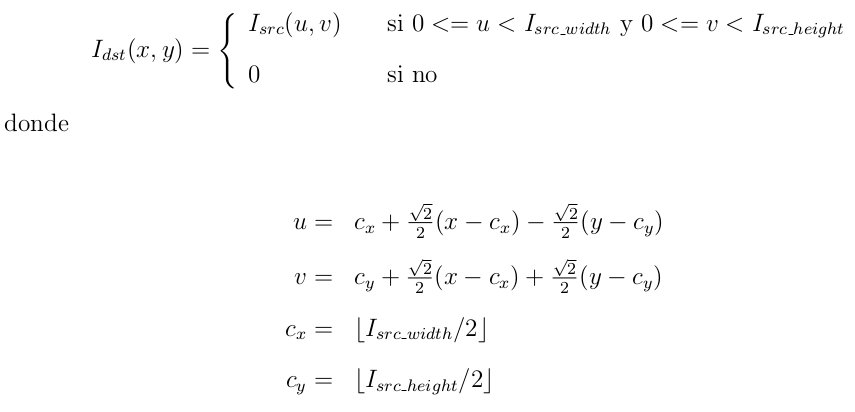
\includegraphics[width=\textwidth]{rotar.jpg} 

\subsubsection{Implementación en C}

La implementación es muy directa con respecto a la especificación. Dos ciclos anidados para recorrer los píxeles destino, y dentro de cada iteración se calculan $u$ y $v$ y se define si se debe colocar un pixel negro o el valor de $I_{src}$(u, v).
Para cada pixel se realiza uno o dos accesos a memoria según corresponda leer o no.

\subsubsection{Implementación en Assembler}

Este filtro tiene ciertas características que impiden aprovechar las operaciones SIMD:
\begin{itemize}
\item Primero, el cálculo de $u$ y $v$ depende de la posición horizontal en la imagen, por lo tanto para calcular 16 píxeles se requieren 16 valores distintos. Esto hace perder la ventaja de realizar varias operaciones en simultáneo ya que cargar 16 valores distintos y luego calcular una sola vez tiene un costo similar a calcular 16 veces. Sin embargo, podría realizarse igualmente (de hecho, algo similar sucede con el filtro waves) de no ser por:
\item Los valores de píxeles consecutivos de la imagen destino dependen de píxeles no consecutivos en la imagen fuente, como puede observarse fácilmente en la imagen de ejemplo. En consecuencia, para escribir 16 píxeles se requiere de 16 lecturas independientes a memoria, arruinando la principal ventaja que estábamos obteniendo con operaciones SIMD.
\end{itemize}

El filtro Rotar, por su forma que lo caracteriza, es incapaz de aprovechar los registros $xmm$ para acceder a memoria efectivamente. Y, aunque por medio dea microoptimizaciones, como prescindir de variables locales en memoria, se podría obtener un mejor resultado que en la versión en C, lo que vimos en los otros filtros demuestra que el principal factor en determinar la eficacia eran los accesos a memoria y cualquier mejora sería despreciable.
Por lo tanto decidimos no implementarlo.